\begin{evenBlock}{HOWTO:  Dribble (5 min)}

\begin{minipage}[t]{\linewidth}
    \centering
    Review these elements prior to beginning the dribbling drills so its fresh in their heads.

    %\begin{minipage}{.3\linewidth} % Left column and width
        %\centering
        %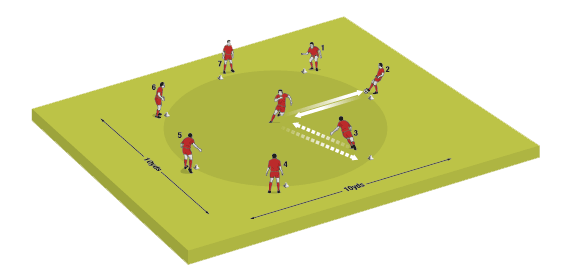
\includegraphics[width=\textwidth]{../img/Trimmed/Clocks1}
    %\end{minipage}
    %\hspace{0.05\linewidth}
    %\begin{minipage}{.6\linewidth} % Left column and width
    
        \textbf{Methods of Dribbling:}
        \begin{enumerate}
        \setlength{\itemsep}{0pt}
        \setlength{\parskip}{0pt}
        \setlength{\parsep}{0pt}
        \item Inside of the foot - used for control, turning.
        \item Outside/Laces of the foot - used for speed and balance.
        \end{enumerate}
        
        Demonstrate running with inside of foot facing forward vs. running with outside or laces forward.

        Have the boys try running both ways and ask which methods allows them to run faster?

    %\end{minipage}
\end{minipage}

\end{evenBlock}